\chapter{Sprints 1 et 2 : Architecture, outils et environnement de développement}
\minitoc
\newpage

\newcommand{\bluecheck}{}%
\DeclareRobustCommand{\greencheck}{%
  \tikz\fill[scale=0.4, color=green]
  (0,.35) -- (.25,0) -- (1,.7) -- (.25,.15) -- cycle;%
}



\section*{Introduction}
\addcontentsline{toc}{section}{Introduction}
Ce chapitre décrit le Sprint zéro, qui constitue la première étape de la réalisation de notre projet SafeTrack. Nous commençons par identifier les différents acteurs de l'application, puis nous listons les besoins fonctionnels et non fonctionnels du système. Ensuite, nous détaillons l'organisation du travail selon la méthodologie Scrum présentée dans le chapitre précédent. Enfin, nous présentons un aperçu du matériel de base, des technologies et des langages de programmation utilisés pour configurer l'environnement de développement.


\section{Capture des besoins}

\subsection{Identification des acteurs}

L'application SafeTrack se compose de trois types d'utilisateurs principaux : Administrateur, organisation et Utilisateur, chacun ayant des rôles et responsabilités spécifiques.

\subsubsection*{Administrateur}
L'administrateur est responsable de la supervision globale de la plateforme. Il a un contrôle complet sur les utilisateurs, les alertes et les statistiques. Ses responsabilités incluent :
\begin{itemize}
    \item Gestion des comptes utilisateurs et des organisations
    \item Consultation des historiques de déplacements et des rapports statistiques
    \item Accès aux visualisations et tableaux de bord
\end{itemize}



\subsection*{Organisation}
Les organisations (écoles, maisons de retraite, centres de soins) utilisent SafeTrack pour suivre les personnes sous leur responsabilité. Elles peuvent :
\begin{itemize}
    \item Gérer et suivre les utilisateurs qui leur sont attribués
    \item Vérifier les trajets et déplacements (ex. transport scolaire ou déplacements des résidents)
    \item Recevoir et gérer les alertes liées aux utilisateurs
\end{itemize}
\newpage

\subsection*{Utilisateur}
L'utilisateur peut être une personne dépendante (enfant, personne âgée) ou son aidant/parent. Leurs capacités diffèrent selon le rôle :

\textbf{Aidant / Parent :}
\begin{itemize}
    \item Visualiser la position en temps réel de la personne dépendante
    \item Définir et gérer des zones sécurisées
    \item Accéder à l'historique de déplacements de la personne dépendante sous sa responsabilité
    \item Recevoir des notifications et des alertes SOS
\end{itemize}

\textbf{Personne Dépendante (Enfant, Personne âgée) :}
\begin{itemize}
    \item Visualiser leur propre position en temps réel
    \item Envoyer des alertes SOS en cas de danger
    \item Recevoir des notifications
    \item Interagir avec le système sans accès administratif global
\end{itemize}

\subsection{Besoins fonctionnels}

Les besoins fonctionnels décrivent les actions attendues de chaque acteur de l'application SafeTrack, en termes de suivi, sécurité et communication.

\subsubsection*{Pour l'Administrateur}
\begin{itemize}
    \item Gérer les comptes utilisateurs et les organisations (ajouter, supprimer, modifier)
    \item Consulter les historiques de déplacements et générer des rapports statistiques
    \item Accéder aux tableaux de bord pour visualiser l'activité globale et les performances du système
\end{itemize}


\subsection*{Pour l'Organisation (écoles, maisons de retraite, centres de soins)}
\begin{itemize}
    \item Suivre les utilisateurs sous leur responsabilité en temps réel
    \item Gérer et organiser les trajets (ex. transport scolaire, déplacements des résidents)
    \item Recevoir et traiter les alertes liées aux utilisateurs
    \item Consulter l'historique de déplacements et les rapports pour optimiser la sécurité
\end{itemize}

\subsection*{Pour l'Aidant / Parent}
\begin{itemize}
    \item Visualiser la position en temps réel de la personne dépendante sous sa responsabilité
    \item Définir et gérer des zones sécurisées (domicile, école, centre de soins, etc.)
    \item Consulter l'historique de déplacements de la personne dépendante sous sa responsabilité
    \item Recevoir des notifications et des alertes SOS
    \item Passer automatiquement des appels d'urgence aux contacts de confiance en cas d'alerte
\end{itemize}

\subsection*{Pour la Personne Dépendante (Enfant, Personne âgée)}
\begin{itemize}
    \item Visualiser leur propre position en temps réel
    \item Envoyer des alertes SOS en cas d'urgence avec localisation exacte
    \item Recevoir des notifications et alertes liées à la sécurité et aux situations à risque
    \item Interagir avec le système sans accès administratif global
\end{itemize}

\subsection{Besoins non fonctionnels}

Les besoins non fonctionnels décrivent les critères qualitatifs essentiels pour garantir une expérience utilisateur optimale et le bon fonctionnement de l'application \textbf{SafeTrack}.

\begin{itemize}
    \item \textbf{Performance :} L'application doit mettre à jour la position des utilisateurs en temps réel et envoyer les alertes sans latence notable, même avec un grand nombre d'utilisateurs simultanés.
    
    \item \textbf{Fiabilité :} L'application doit être stable et exempte de bugs. En cas de problème technique, elle doit pouvoir se rétablir rapidement avec un minimum d'impact pour les utilisateurs.
    
    \item \textbf{Sécurité :} Les données personnelles et sensibles doivent être protégées par chiffrement. Les connexions doivent utiliser des protocoles sécurisés (HTTPS) et la gestion des identifiants (JWT) doit empêcher tout accès non autorisé.RBAC (Role-Based Access Control) doit être mis en place pour garantir que les utilisateurs n'accèdent qu'aux fonctionnalités et données qui leur sont autorisées.
    
    \item \textbf{Scalabilité :} L'application doit pouvoir évoluer facilement pour gérer l'augmentation du nombre d'utilisateurs et de données. L'utilisation de conteneurs (Docker) permet de dupliquer les services et d'assurer une montée en charge fluide et contrôlée.
    
    \item \textbf{Maintenabilité :} Le code doit être bien structuré, documenté et facile à maintenir, facilitant ainsi les futures mises à jour et évolutions.
    
    \item \textbf{Compatibilité :} L'application doit être compatible avec les principaux systèmes d'exploitation mobiles (Android, iOS) et navigateurs Web (Chrome, Firefox, Safari), ainsi qu'avec les plateformes Windows, macOS et Linux pour le dashboard.
    
    \item \textbf{Disponibilité :} L'application doit être opérationnelle 24h/24 et 7j/7 pour garantir la sécurité des utilisateurs vulnérables.
\end{itemize}

\section{Product Backlog}
À cette étape, en jouant le rôle de Product Owner (PO) et en s'appuyant sur l'analyse des besoins présentée précédemment, il est essentiel de préparer le Product Backlog. Celui-ci regroupe toutes les fonctionnalités attendues sous forme de Product Backlog Items (PBI). Chaque PBI reflète un besoin des utilisateurs ou des parties prenantes, et peut être exprimé sous forme de User Stories pour faciliter la compréhension et la planification.

Pour le projet SafeTrack, les PBI incluent par exemple : le suivi en temps réel, la gestion des zones sécurisées, les alertes SOS, l'historique des déplacements et l'intégration de l'intelligence artificielle pour la détection des situations à risque.

Il est également important, à ce stade, de définir une technique de priorisation du Product Backlog afin de déterminer quelles fonctionnalités doivent être développées en premier, en fonction de leur valeur pour les utilisateurs et de leur impact sur la sécurité et l'efficacité de l'application.
\small
\renewcommand{\arraystretch}{1.2}
\begin{longtable}{|>{\raggedright\arraybackslash}p{0.27\textwidth}|>{\raggedright\arraybackslash}p{0.58\textwidth}|>{\centering\arraybackslash}p{0.09\textwidth}|}
\caption{Product Backlog} \label{tab:product_backlog} \\
\hline
\textbf{Groupe de Fonctionnalités} & \textbf{User Stories} & \textbf{Priorité}  \\
\hline
\endfirsthead
\caption[]{Product Backlog (suite)} \\
\hline
\textbf{Groupe de Fonctionnalités} & \textbf{User Stories} & \textbf{Priorité}  \\
\hline
\endhead
\hline
\endfoot
\hline
\endlastfoot
\hline

Authentification et Gestion des Utilisateurs 
& En tant que parent, aidant ou organisation, je peux créer un compte afin d'accéder à la plateforme SafeTrack et gérer mes responsabilités. 
& Haute \\
\cline{2-3}
& En tant qu'utilisateur autorisé, je peux m'authentifier de manière sécurisée afin d'accéder à mon espace personnel. 
& Haute \\
\cline{2-3}
& En tant qu'administrateur, je peux consulter, modifier ou supprimer des comptes utilisateurs afin d'assurer la gestion globale du système. 
& Haute \\
\hline

Gestion des Profils (Enfants et Personnes à‚gées) 
& En tant que parent ou aidant, je peux créer et gérer des profils pour des enfants ou des personnes âgées dépendantes afin d'assurer leur suivi. 
& Haute \\
\cline{2-3}
& En tant que parent ou aidant, je peux associer un profil à une organisation (école, centre de soins) ou choisir de ne pas l'associer. 
& Haute \\
\hline

Suivi en Temps Réel 
& En tant que parent, aidant ou organisation, je peux visualiser la localisation des profils suivis en temps réel sur une carte interactive. 
& Haute \\
\cline{2-3}
& En tant qu'utilisateur, je peux recevoir des notifications en temps réel lors de changements significatifs de position. 
& Haute \\
\cline{2-3}
& En tant qu'utilisateur, je peux activer un mode économie de batterie pour réduire la fréquence d'envoi de position. 
& Basse \\
\hline

Zones Sécurisées (Geofencing) 
& En tant que parent ou aidant, je peux définir des zones sécurisées (domicile, école, centre de soins) afin de surveiller les déplacements. 
& Haute \\
\cline{2-3}
& En tant qu'utilisateur, je peux recevoir des alertes lorsque le profil suivi entre ou sort d'une zone sécurisée. 
& Haute \\
\hline

Historique des Déplacements 
& En tant que parent, aidant ou organisation, je peux consulter l'historique des déplacements afin d'analyser les trajets et comportements passés. 
& Moyenne \\
\cline{2-3}
& En tant qu'administrateur, je peux exporter l'historique en PDF ou CSV pour archivage. 
& Basse \\
\hline

Alertes SOS et Gestion des Urgences 
& En tant que parent ou aidant, je peux recevoir une alerte SOS avec la localisation en temps réel afin d'intervenir rapidement en cas de danger. 
& Haute \\
\cline{2-3}
& En tant qu'personne dépendante ou personne âgée suivie, je peux déclencher un appel d'urgence afin de contacter rapidement mes proches ou aidants en situation critique. 
& Haute \\
\cline{2-3}
& En tant qu'utilisateur, je peux activer une alerte discrète (mode silencieux) en situation sensible. 
& Basse \\
\hline

Intelligence Artificielle (RAG + LLM) 
& En tant que système SafeTrack, je peux analyser les données de localisation pour détecter des anomalies et prioriser les alertes SOS. 
& Haute \\
\cline{2-3}
& En tant que parent, aidant ou organisation, je peux recevoir des alertes intelligentes, des ETA et des recommandations de zones sures. 
& Haute \\
\cline{2-3}
& En tant que parent, je peux ajuster le niveau de sensibilité de la détection d'anomalies selon le profil suivi. 
& Basse \\
\hline

Tableau de Bord (Administration et organisations) 
& En tant qu'administrateur ou organisation, je peux consulter un tableau de bord affichant des statistiques et visualisations afin de superviser l'activité globale des utilisateurs. 
& Haute \\
\hline

\end{longtable}
\normalsize



Le Product Backlog représente un élément central de la méthodologie agile utilisée pour le développement de SafeTrack. Il compile, sous forme de liste priorisée, toutes les fonctionnalités, améliorations et corrections à apporter à l'application, appelées user stories. Chaque user story décrit une fonctionnalité spécifique, précise les critères d'acceptation et fournit une estimation de l'effort nécessaire à sa réalisation. Ce document est évolutif et est régulièrement mis à jour tout au long du projet, afin de garantir que l'équipe se concentre constamment sur les tâches les plus importantes et les plus pertinentes pour atteindre les objectifs fixés.
\section{Les Diagrammes }
\subsection{Diagramme de cas d'utilisation global}
Le diagramme de cas d'utilisation est un outil clé pour représenter les interactions entre les différents acteurs et le système. Il fournit une vue d'ensemble des actions réalisables par les utilisateurs, notamment les utilisateurs finaux, les organisations et l'administrateur. Ce diagramme met en avant les principales fonctionnalités de l'application et montre comment chaque acteur les utilise. Il facilite la compréhension des échanges entre le système et ses utilisateurs, tout en permettant d'identifier d'éventuelles lacunes ou incohérences dans le fonctionnement global de SafeTrack.
\begin{figure}[H]
\centering
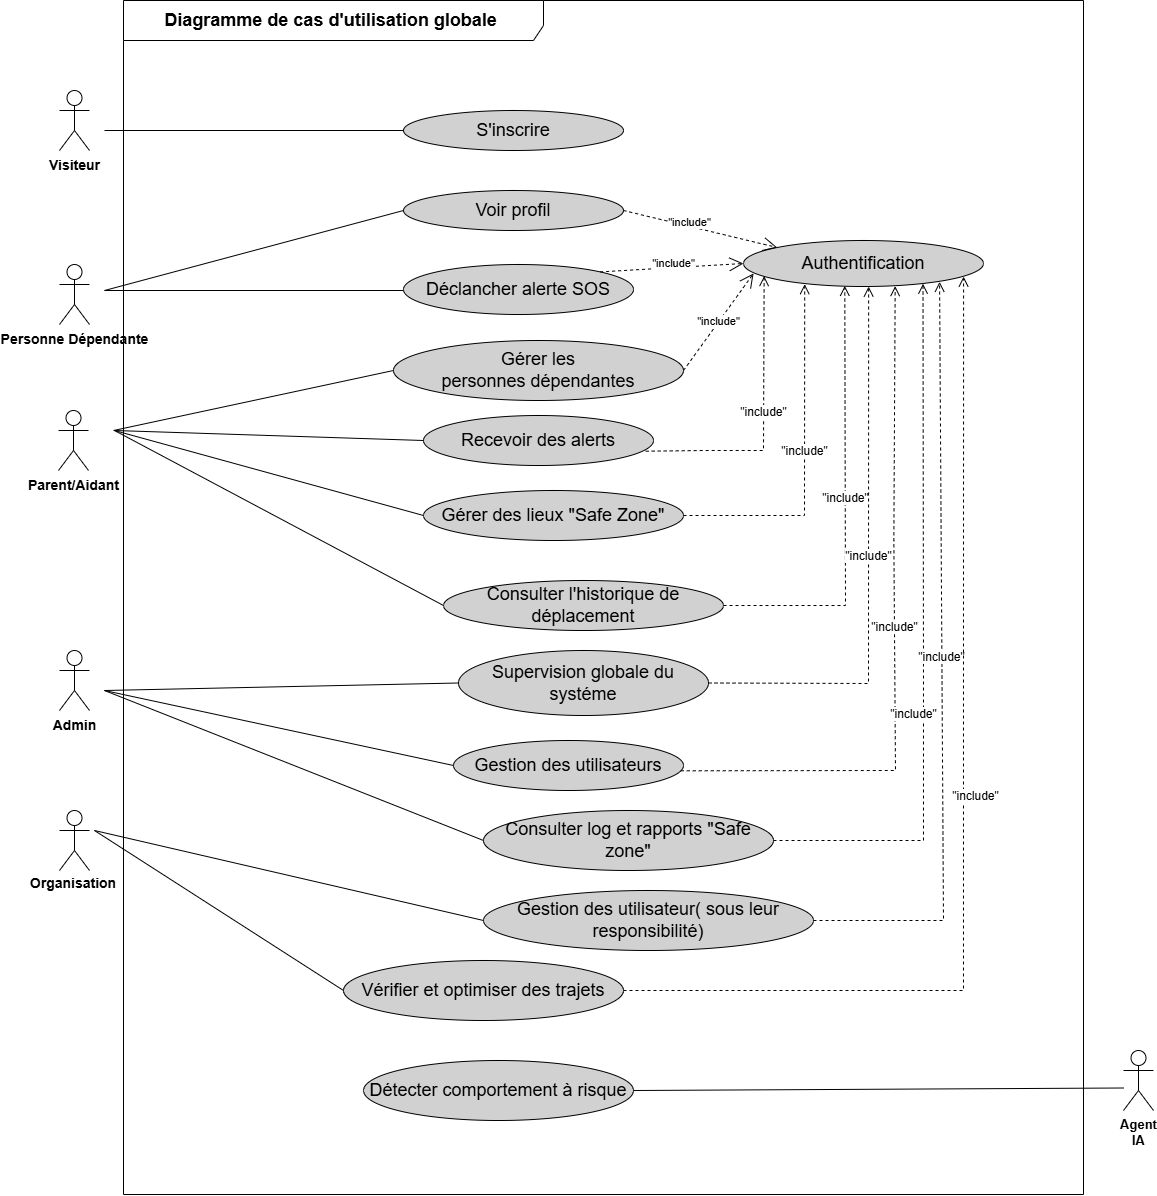
\includegraphics[width=1\columnwidth, height=0.95\textheight]{images/uc globale finale.png}
\caption{Diagramme des cas d'utilisation global}
\label{fig_useCase_global}
\end{figure}
\subsection{Diagramme de classes global}
Le diagramme de classes constitue un élément central de la documentation de conception. Il illustre la structure du système en présentant les classes, leurs attributs et méthodes, ainsi que les relations qui les lient. Ce diagramme sert de plan pour le développement du code, en clarifiant la manière dont les différentes parties de l'application interagissent. Il permet de s'assurer que la conception est cohérente, logique et bien organisée, facilitant ainsi la phase de mise en œuvre de SafeTrack.
\begin{figure}[H]
\centering
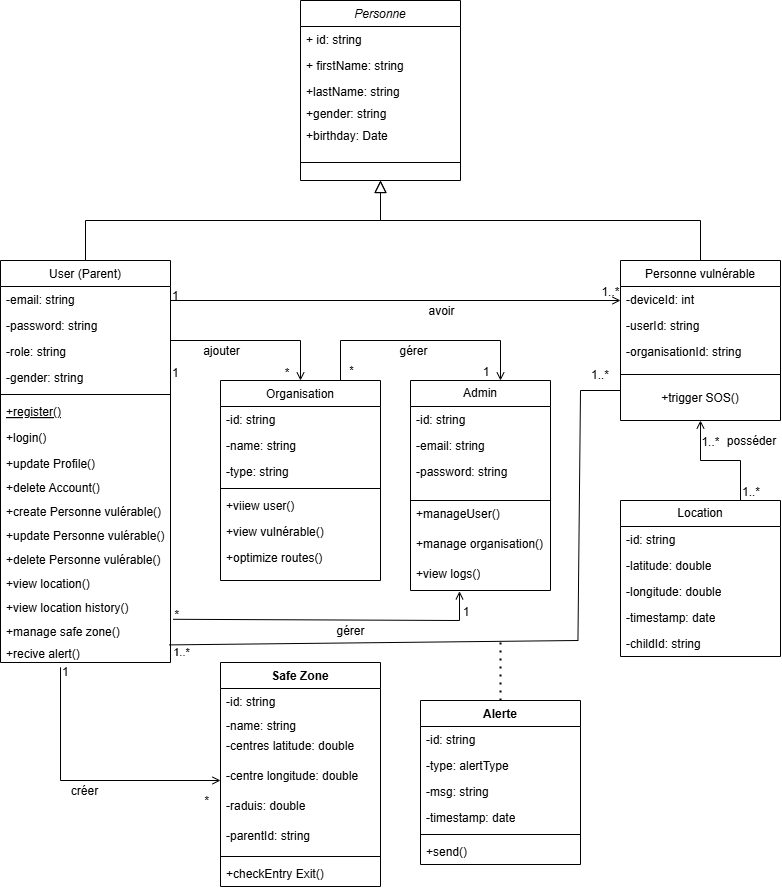
\includegraphics[width=1\columnwidth, height=1\textheight]{images/globaleclasse_diagram.drawio.png}
\caption{Diagramme de classes global }
\label{fig_classes_global}
\end{figure}

\section{Architecture de l'application}

Dans le cadre du projet SafeTrack, nous avons adopté une architecture client--serveur modulaire basée sur des services spécialisés afin de garantir la scalabilité, la sécurité, la maintenabilité et l'évolutivité du système. Cette architecture permet de séparer les différentes responsabilités applicatives tout en facilitant l'intégration de nouvelles fonctionnalités, notamment celles basées sur l'intelligence artificielle.

L'écosystème SafeTrack est constitué de quatre composants principaux :

\begin{itemize}
    \item Une application mobile développée avec \textbf{Flutter} destinée aux parents, aux personnes dépendantes et aux responsables autorisés ;
    
    \item Une application web d'administration développée avec \textbf{React} permettant la gestion centralisée des utilisateurs, des organisations et des données de sécurité ;
    
    \item Un backend principal développé avec \textbf{NestJS} et \textbf{Node.js} assurant la gestion de la logique métier, des données et des communications temps réel ;
    
    \item Un microservice d'intelligence artificielle développé avec \textbf{Python}, \textbf{FastAPI} et une architecture \textbf{RAG (Retrieval-Augmented Generation)}, chargé de l'analyse intelligente des incidents et de la génération de recommandations contextuelles.
\end{itemize}

L'application mobile constitue l'interface principale utilisée par les utilisateurs finaux. Elle permet notamment de consulter la position en temps réel, de recevoir des notifications de sécurité, de gérer les zones sécurisées, d'envoyer des alertes SOS et d'accéder aux fonctionnalités de suivi et de partage de localisation.

L'application web est destinée principalement aux administrateurs et aux organisations partenaires telles que les écoles, les centres de soins ou les associations. Elle offre des outils de supervision permettant la gestion des utilisateurs, le suivi des déplacements, la consultation des alertes, l'administration des \textit{Zones de sécurité} ainsi que la génération de rapports statistiques.

Le backend NestJS constitue le cœur du système. Il expose un ensemble d'API REST sécurisées ainsi que des services de communication temps réel via \textbf{Socket.IO}. Il centralise les traitements métier, assure la gestion des utilisateurs et orchestre les échanges entre les différents composants de la plateforme.

Le backend est organisé selon une architecture modulaire où chaque module est responsable d'un domaine fonctionnel spécifique :

\begin{itemize}
    \item \textbf{Module d'authentification} : gestion de l'inscription, de la connexion, des rôles et de la sécurité des comptes ;
    
    \item \textbf{Module de suivi de localisation} : réception et traitement des positions GPS en temps réel ;
    
    \item \textbf{Module Zone de sécurité} : gestion des zones géographiques sécurisées et détection des sorties ou entrées non autorisées ;
    
    \item \textbf{Module SOS} : gestion des alertes d'urgence et des procédures d'escalade ;
    
    \item \textbf{Module Historique} : stockage et consultation des déplacements ;
    
    \item \textbf{Module Partage} : gestion des autorisations d'accès à la localisation ;
    
    \item \textbf{Module Alertes} : création, diffusion et suivi des notifications de sécurité ;
    
    \item \textbf{Module Administration} : supervision globale de la plateforme.
\end{itemize}

Afin d'améliorer les capacités d'analyse et d'assistance à la décision, SafeTrack intègre également un microservice d'intelligence artificielle indépendant. Ce microservice communique avec le backend via des API dédiées et assure plusieurs fonctions avancées :

\begin{itemize}
    \item Analyse intelligente des incidents de sécurité ;
    
    \item Détection des situations à risque à partir des données de localisation ;
    
    \item Génération de recommandations contextuelles grâce à l'approche RAG ;
    
    \item Production de rapports de sécurité enrichis ;
    
    \item Analyse comportementale et détection d'anomalies de déplacement.
\end{itemize}

Cette séparation sous forme de microservice permet d'isoler les traitements IA du backend principal, d'améliorer la scalabilité du système et de faciliter l'évolution future des modèles d'intelligence artificielle.

Pour la persistance des données, SafeTrack utilise \textbf{MongoDB}, une base de données NoSQL particulièrement adaptée au stockage des informations géographiques, des historiques de déplacement et des données utilisateurs. \textbf{Redis} est utilisé comme système de cache afin d'optimiser les performances des traitements temps réel et la gestion des positions actives.

La sécurité des échanges est assurée par l'utilisation des \textbf{JSON Web Tokens (JWT)}. Après authentification, chaque utilisateur reçoit un jeton sécurisé qui doit être présenté lors des appels aux API. Ce mécanisme permet de contrôler l'accès aux ressources et de garantir l'intégrité des communications.

La localisation en temps réel constitue l'une des fonctionnalités centrales de SafeTrack. Les positions GPS collectées par l'application mobile sont transmises au backend, stockées dans la base de données puis diffusées instantanément aux utilisateurs autorisés grâce aux mécanismes de communication temps réel. Cette approche permet un suivi fiable et réactif des personnes dépendantes.

Enfin, afin de faciliter le déploiement et la portabilité de la solution, les différents services (backend, microservice IA, base de données et cache) peuvent être conteneurisés à l'aide de \textbf{Docker}. Cette approche garantit la cohérence des environnements entre les phases de développement, de test et de production.

Grâce à cette architecture client--serveur modulaire enrichie par un microservice d'intelligence artificielle, SafeTrack offre une plateforme performante, sécurisée et évolutive permettant d'assurer la protection, le suivi et l'assistance intelligente des personnes dépendantes.

\begin{figure}[H]
    \centering
    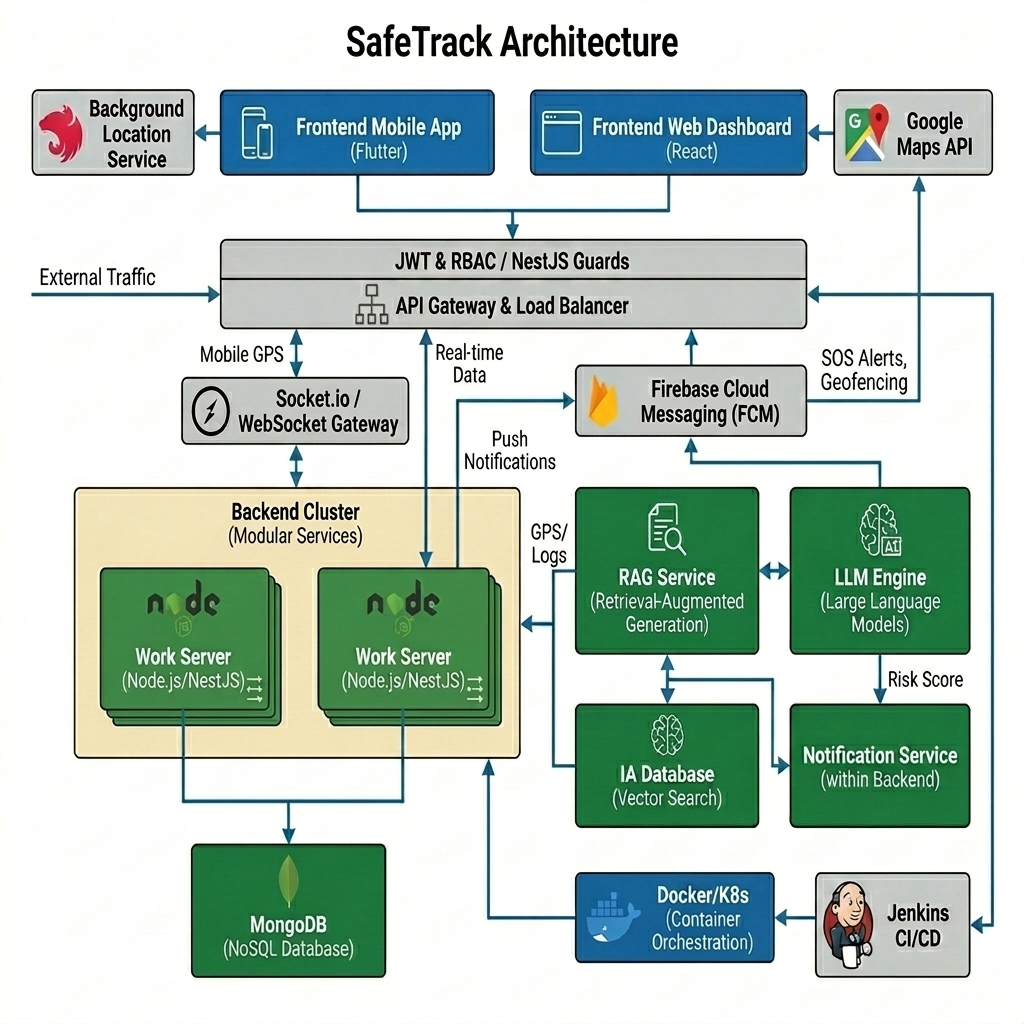
\includegraphics[width=\textwidth]{images/update_the_architecture_diagram_data_image_image_7_for_safetrack_architecture..png}
    \caption{Architecture proposée pour la plateforme}
    \label{fig_architecture_physique}
\end{figure}





\section{Outils et environnement de développement}

\subsection{Environnement matériel}

Dans le cadre de ce projet, plusieurs machines ont été utilisées pour le développement et les tests. Voici les caractéristiques principales des équipements utilisés :

\begin{itemize}
\item[$\bullet$] PC 1 (ASUS Vivobook) :
\begin{itemize}
\item Carte graphique : 128 MB intel(R) UHD Graphics
\item Mémoire RAM : 16 Go
\item Disque : 477GB
\end{itemize}

\item[$\bullet$] PC 2 (Lenovo LOQ) :
\begin{itemize}
    \item Carte graphique : NIVIDIA GeForce RTX 3050 6 GB
    \item Mémoire RAM : 16 Go
    \item Disque : 477 GB
\end{itemize}
\end{itemize}

\subsection{Environnement technique}

\begin{longtable}{| m{2.5cm} | m{13cm} |}
\hline
\textbf{Logo} & \textbf{Outil et Description} \\
\hline
\endfirsthead
\hline
\textbf{Logo} & \textbf{Outil et Description (suite)} \\
\hline
\endhead
\hline
\endfoot
\hline
\endlastfoot

\includegraphics[width=1.5cm]{images/nestjs.png} & 
\textbf{NestJS : \cite{nestjs}}  
Framework backend basé sur Node.js permettant de développer des API REST robustes et structurées grâce à une architecture modulaire inspirée du modèle MVC.
\\
\hline


\includegraphics[width=1.5cm]{images/react.png} & 
\textbf{React.js : \cite{reactjs}}  
Bibliothèque JavaScript utilisée pour le développement de l'application web (dashboard), offrant une interface interactive et dynamique pour la gestion et la supervision des utilisateurs.
\\
\hline


\includegraphics[width=1.5cm]{images/flutter.png} & 
\textbf{Flutter : \cite{flutter}}  
Framework multiplateforme utilisé pour le développement de l'application mobile, permettant une expérience utilisateur fluide sur Android et iOS.
\\
\hline


\includegraphics[width=1.5cm]{images/nodejs.png} & 
\textbf{Node.js : \cite{nodejs}}  
Environnement d'exécution JavaScript côté serveur utilisé pour le développement du backend.
\\
\hline


\includegraphics[width=1.5cm]{images/mongodb.png} & 
\textbf{MongoDB : \cite{mongodb}}  
Base de données NoSQL utilisée pour stocker les informations des utilisateurs ainsi que les données de géolocalisation en temps réel.
\\
\hline


\includegraphics[width=1.2cm]{images/redis.png} & 
\textbf{Redis : }  
Base de données en mémoire utilisée comme système de cache et de gestion des données en temps réel.
\\
\hline


\includegraphics[width=1.5cm]{images/ioredis.png} & 
\textbf{ioredis : \cite{ioredis}}  
Client Redis utilisé pour la gestion du cache et la communication temps réel entre services.
\\
\hline


\includegraphics[width=1.2cm]{images/websocket.png} & 
\textbf{Socket.IO : }  
Bibliothèque permettant une communication bidirectionnelle et en temps réel entre les clients et le serveur.
\\
\hline


\includegraphics[width=1cm]{images/jwt.png} & 
\textbf{JWT : }  
Standard utilisé pour l'échange sécurisé de jetons d'authentification entre les différentes parties du système.
\\
\hline


\includegraphics[width=1.2cm]{images/firebaselogo.png} & 
\textbf{Firebase Cloud Messaging (FCM) : }  
Service utilisé pour l'envoi de notifications push instantanées sur les appareils mobiles.
\\
\hline


\includegraphics[width=1.5cm]{images/mapslogo.png} & 
\textbf{Google Maps API : }  
Service de cartographie utilisé pour visualiser la localisation des utilisateurs et gérer les zones sécurisées.
\\
\hline


\includegraphics[width=1.8cm]{images/swaggerlogo.png} & 
\textbf{Swagger (OpenAPI) : }  
Documentation et test interactif des API REST du backend.
\\
\hline


\includegraphics[width=1.2cm]{images/ollama.jpeg} & 
\textbf{Ollama : }  
Exécution locale des modèles de langage utilisés par le système RAG pour l'analyse et la génération de recommandations.
\\
\hline


\includegraphics[width=1.2cm]{images/chromadblogo.png} & 
\textbf{ChromaDB : }  
Base de données vectorielle utilisée par le système RAG pour stocker et rechercher les connaissances contextuelles.
\\
\hline


\includegraphics[width=1.5cm]{images/bcryptlogo.jpg} & 
\textbf{bcrypt : }  
Hachage et sécurisation des mots de passe avant leur stockage dans la base de données.
\\
\hline


\includegraphics[width=1.5cm]{images/docker.png} & 
\textbf{Docker \& Docker Compose : \cite{docker}}  
Utilisés pour la conteneurisation des services et la gestion des environnements de déploiement.
\\
\hline


\includegraphics[width=0.8cm]{images/gitlab.jpg}

\includegraphics[width=0.8cm]{images/github.png} & 
\textbf{GitLab \& GitHub : \cite{github} \cite{gitlab}}  
Outils de gestion de version et de collaboration permettant le suivi du code source ainsi que l'intégration continue (CI/CD).
\\
\hline


\includegraphics[width=1.5cm]{images/vscode.png} & 
\textbf{Visual Studio Code : \cite{vscode}}  
Éditeur de code utilisé pour le développement grâce à ses nombreuses extensions.
\\
\end{longtable}









\section*{Conclusion}
\addcontentsline{toc}{section}{Conclusion}
En conclusion, Ce chapitre a posé les bases de notre projet en identifiant les acteurs, les besoins fonctionnels et non fonctionnels, et en élaborant un Product Backlog détaillé. Les diagrammes UML ont facilité la compréhension de l'architecture de l'application, tandis que le choix des technologies adaptées a permis de garantir une solution à la fois performante et sécurisée. Les outils et l'environnement de développement sélectionnés ont optimisé notre productivité et préparent efficacement les prochaines étapes de mise en œuvre présentées dans les chapitres suivants.
\enlargethispage{2\baselineskip}

